\documentclass[11pt]{article}

\usepackage[margin=1in]{geometry}
\usepackage{amsmath,amssymb,amsthm}
\usepackage{graphicx}
\usepackage[hidelinks]{hyperref}

\newtheorem{theorem}{Theorem}
\newtheorem{lemma}{Lemma}

\DeclareMathOperator{\spanop}{span}

\title{Removing Completeness from the Metric \(C_b(K)\) Invariant-Subspace Classification}
\author{Run \texttt{fa\_banach\_001}, agent \texttt{agent\_lane\_19}}
\date{June 15, 2026}

\begin{document}
\maketitle

\section*{Status}

This is a partial/theorem-adjacent result for Cheng--Fang--Jiang,
\emph{On the third problem of Halmos on Banach spaces}, arXiv:2203.14670v2
\cite{CFJ}.  It does not solve Halmos's third problem for invertible operators.
It strengthens the final \(C(K)\)-classification in the source paper by
removing the assumption that the metric space \(K\) is complete.

\section*{Source Passage}

The source paper writes \(C(K)\) for the Banach space of bounded continuous
complex-valued functions on a metric space \(K\), with the supremum norm.
Theorem 16.1 assumes that \(K\) is complete:

\begin{center}

\includegraphics[width=\textwidth]{figures/open_problem_crop.png}
\end{center}

In the proof tail, completeness is used only in the noncompact case:

\begin{center}
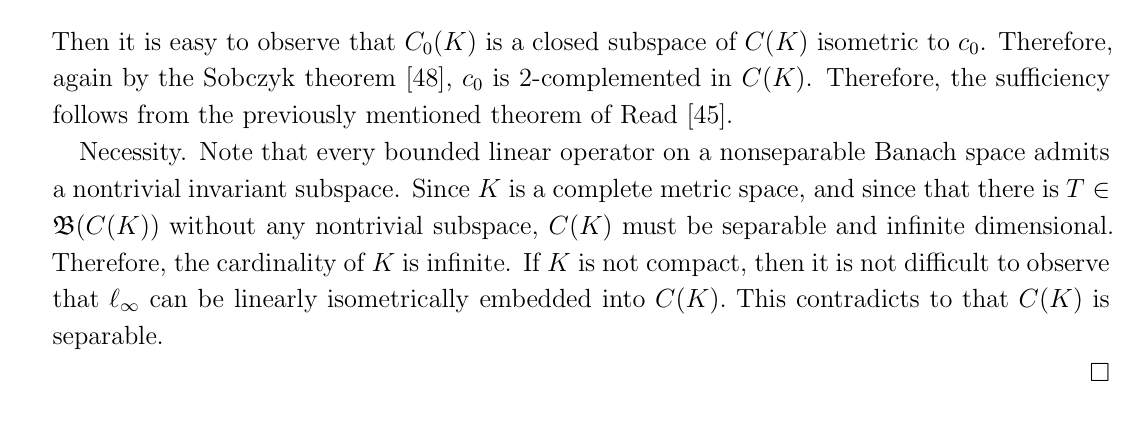
\includegraphics[width=\textwidth]{figures/source_proof_tail_crop.png}
\end{center}

\section*{Claim}

Let \(K\) be a metric space and let \(C_b(K)\) denote the Banach space of
bounded continuous complex-valued functions on \(K\), with the supremum norm.
Assume \(C_b(K)\) is infinite-dimensional. Then \(C_b(K)\) admits a bounded
linear operator without nontrivial closed invariant subspaces if and only if
\(K\) is compact.

\section*{Proof Intuition}

The compact side needs no new work: compact metric spaces are complete, so the
source theorem applies directly.  The only issue is whether a noncomplete,
noncompact metric space might evade the source paper's necessity argument.
It cannot.  Every noncompact metric space contains a closed discrete infinite
sequence.  Restricting bounded continuous functions to that sequence gives a
quotient map from \(C_b(K)\) onto \(\ell_\infty\), by Tietze extension.  Thus
\(C_b(K)\) is nonseparable, and on a nonseparable Banach space every operator
has a nontrivial invariant subspace: the closed orbit generated by one nonzero
vector is separable.

\section*{Proof}

We use two elementary facts.

\begin{lemma}\label{lem:nonsep}
Let \(X\) be a nonseparable Banach space.  Then every \(T\in\mathcal B(X)\)
has a nontrivial closed invariant subspace.
\end{lemma}

\begin{proof}
Choose \(0\neq x\in X\).  The closed linear span
\[
  M=\overline{\spanop}\{x,Tx,T^2x,\ldots\}
\]
is a nonzero closed \(T\)-invariant subspace.  It is separable.  Since \(X\) is
nonseparable, \(M\neq X\).
\end{proof}

\begin{lemma}\label{lem:cbnonsep}
If \(K\) is a noncompact metric space, then \(C_b(K)\) is nonseparable.
\end{lemma}

\begin{proof}
Since metric compactness is equivalent to sequential compactness, there is a
sequence \((x_n)\) in \(K\) with no convergent subsequence.  Passing to a
subsequence if needed, assume the \(x_n\)'s are distinct, and put
\(D=\{x_n:n\geq 1\}\).

The set \(D\) is closed and discrete in \(K\).  Indeed, any accumulation point
of \(D\) would be the limit of a subsequence of \((x_n)\).  Hence every bounded
function on \(D\) is continuous, so \(C_b(D)\) is isometric to \(\ell_\infty\).
The restriction operator
\[
  R:C_b(K)\longrightarrow C_b(D),\qquad Rf=f|_D,
\]
is bounded and linear.  It is onto by the Tietze extension theorem, because
metric spaces are normal and \(D\) is closed.  Therefore \(\ell_\infty\) is a
continuous linear image of \(C_b(K)\).  If \(C_b(K)\) were separable, then
\(\ell_\infty\) would be separable, a contradiction.
\end{proof}

Now suppose first that \(K\) is compact and \(C_b(K)\) is infinite-dimensional.
Then \(K\) is a complete metric space, and Theorem 16.1 of \cite{CFJ} gives a
bounded operator on \(C_b(K)=C(K)\) without nontrivial closed invariant
subspaces.

Conversely, suppose that \(K\) is not compact.  By Lemma \ref{lem:cbnonsep},
\(C_b(K)\) is nonseparable.  Lemma \ref{lem:nonsep} then implies that every
bounded operator on \(C_b(K)\) has a nontrivial closed invariant subspace.  So
no bounded operator without nontrivial closed invariant subspaces exists on
\(C_b(K)\).

This proves the equivalence for arbitrary metric spaces \(K\).

\section*{Verification and Limitations}

The proof is independent of the difficult Read construction except through the
compact-metric sufficiency already proved in the source paper.  The new
necessity argument uses only the standard facts that noncompact metric spaces
are not sequentially compact, metric spaces are normal, and Tietze extension
holds for bounded scalar-valued continuous functions on closed subsets.

This packet does not answer the source paper's main Halmos Problem 1.2.  It
only removes an unnecessary completeness assumption from the source paper's
final \(C(K)\) theorem.

Local run indexes were searched for the arXiv id and keywords
\(\texttt{C(K)}\), \(\texttt{C\_b(K)}\), \(\texttt{complete metric}\),
\(\texttt{bounded continuous}\), and invariant-subspace terms.  Web searches
were run for the Halmos third problem and for \(C_b(X)\) noncompact metric
separability variants.  No duplicate run packet or explicit later literature
answer for this exact strengthening was found.  Since the new step is
standard-topology folklore-level, human review should treat the novelty claim
conservatively.

\section*{Human Review Recommendation}

Check that the source paper's \(C(K)\) notation indeed means \(C_b(K)\) for
noncompact metric spaces, as stated in Theorem 16.1.  Then verify the
restriction/Tietze quotient argument in Lemma \ref{lem:cbnonsep}.  If accepted,
the source theorem can be restated for all metric spaces.

\begin{thebibliography}{9}

\bibitem{CFJ}
Lixin Cheng, Junsheng Fang, Chunlan Jiang,
\emph{On the third problem of Halmos on Banach spaces},
arXiv:2203.14670v2, 2022.

\bibitem{Tietze}
Heinrich Tietze,
\emph{Ueber Funktionen, die auf einer abgeschlossenen Menge stetig sind},
Journal fuer die reine und angewandte Mathematik \textbf{145} (1915), 9--14.

\end{thebibliography}

\end{document}
